%%%%%%%%%%%%%%%%%%%%%%%%%%%%%%%%%%%%%%%%%%%%%%%
%
%   Families of Traffic Forecasting Problems
%
%%%%%%%%%%%%%%%%%%%%%%%%%%%%%%%%%%%%%%%%%%%%%%%

%\usepackage{cite}
%\usepackage{multirow}
%\usepackage{rotating} 
%\usepackage[table,xcdraw]{xcolor}
%\usepackage{float}
%\usepackage[utf8]{inputenc}
%\usepackage{amsmath,amssymb,amsfonts}
%\usepackage{algorithmic}
%\usepackage{graphicx}
%\usepackage{textcomp}
%\usepackage{rotating}
%\usepackage{verbatim}


\section{Experimental Results}
\label{sec:4_5_Expsetup}

The objective of the experiments conducted in this study was to evaluate the efficacy of multiclass oversampling techniques in enhancing the performance of the first proposed method in imbalanced drifted multiclass classification streams. Our primary goal was to develop a novel approach that combines Dynamic Ensemble Selection (DES) to improve classification accuracy and robustness in such streams. These experiments yielded valuable insights that could further refine the performance of the first proposed approach and its ability to effectively handle imbalanced data streams. These findings provide a better understanding of the capabilities of the first proposed approach and offer insights into an optimal strategy for tackling minority class issues and concept drift in imbalanced data streams. This study contributes to the advancement of stream mining techniques for generating more accurate and robust classification models in dynamic data stream environments. By addressing the challenges posed by minority classes and concept drift, this study offers valuable insights for improving the performance of the first proposed approach and enhancing the overall efficiency of stream mining. The two main questions to be answered are:

\begin{itemize}
  % \setlength{\itemindent}{-.5in}
  
      \item $\pmb{Q_1}$: What is the impact of reduced and consistent data on the performance of ensemble learning?
      \item  $\pmb{Q_2}$: Is it possible with the search capability of swarm intelligence to enhance the combination of classifiers? 
  \end{itemize}

\subsection{Experimental setup}
The evaluation of the first proposed approach incorporated the utilization of various metrics such as recall, precision, specificity, f1 score, balanced accuracy score (BAC), and geometric mean score (G-mean) \cite{bu2016pdf}. The experimental protocol utilized for evaluation was the test-then-train approach \cite{venkatasubramanianinformation}, where the classification classifier was trained on a specific data chunk and subsequently evaluated on the subsequent one. The chunk size was standardized for all utilized data streams to 2,000 instances. We employed four classification classifiers as base estimators: K-Nearest Neighbor (KNN), Support Vector Machine (SVM), Gaussian Naive Bayes (GNB), and Hoeffding Tree (HT), as implemented in scikit-learn \cite{frias2014online}. A pool of classifiers was constructed with a maximum size of L = 8, where the DES selected the best classifier for each chunk. If the pool surpassed the set threshold (L), the classifier with the lowest performance was eliminated. The experiments were conducted using Python programming language, and the source code was publicly available on GitHub\footnote{\url{https://github.com/Amadkour/dynamic__classification_ensembles_for_handling_imbalanced_multi-class_drifted_data_streams.git}} . We conducted a comparison between multiclass oversampling techniques (MLSMOTE and MLSOL) and first proposed approach to demonstrate the effectiveness of our contribution. Additionally, we conducted these experiments using two different concept drift detectors, ADWIN \cite{storkey2008training} and DDM \cite{losing2016knn}, to demonstrate the adaptability and robustness of first proposed approach across varying drift detectors.

\subsection{Data Streams}
In this study, the first approach was assessed using various datasets including benchmark datasets, a real application stream dataset, and synthetic data streams. The Stream-learn Python library was used to conduct the evaluations \cite{dries2009adaptive}. Table \ref{tab:4_first_proposal_result_table_1} illustrates the benchmark dataset employed in this study, which consists of the Covertype dataset containing 40 features, seven classes, and 581,010 instances. For real application stream evaluation, the Sensor stream dataset was used, which consisted of five features, 58 classes, and 392,600 instances. This represents a real-world application scenario and provides valuable insights into the performance of the first proposed approach in practical settings. Synthetic datasets were generated using Scikit-learn Python library to evaluate the performance of the first proposed approach. The synthetic dataset was designed to simulate data streams and comprised 10 features and four classes divided into 200 chunks of 2,000 instances each. The performance of the first approach was systematically evaluated using these datasets and a stream-learn library. These evaluations provided insights into the effectiveness of the first approach in handling different types of data streams, including benchmark datasets, real application streams, and synthetic data streams.

\begin{table}[h!]
  \centering
  \caption{Summary of Dataset Characteristics Utilized in the PA1 Experimental.}
  \resizebox{\textwidth}{!}{
  \begin{tabular}{|l|c|c|c|}
  \hline
  \textbf{Dataset} & \textbf{Number of Features} & \textbf{Number of Classes} & \textbf{Number of Instances} \\ \hline
  Covertype dataset\footnote{\url{http://archive.ics.uci.edu/dataset/31/covertype}} & 40 & 7 & 581,010 \\ \hline
  Sensor Stream dataset\footnote{\url{https://www.cse.fau.edu/~xqzhu/Stream/sensor.arff}} & 5 & 58 & 392,600 \\ \hline
  Synthetic stream & 8 & 3 & 200,000 \\ \hline
  \end{tabular}
  }
  \label{tab:4_first_proposal_result_table_1}
  \end{table}

\subsection{Analysis of Experimental Results}
The performance of the first proposed approach was comprehensively assessed on multiple data streams, considering two distinct concept drift detectors, ADWIN and DDM. To ensure thorough evaluation, six key performance metrics—F1 score, recall, precision, G-mean, specificity, and balanced accuracy—were carefully presented using two visualization diagrams: radar and line. A radar diagram was strategically utilized to provide an overview that effectively depicted the performance of each algorithm across the six metrics. The mean value of each metric was calculated to present the overall performance of each method (MLSMOTE, MLSOL, PA1). It is important to note that the PA1 is represented by red lines.

\subsubsection{Results on the Benchmark Stream}
\vspace{-3mm}
\begin{figure}[H]
	\centering
	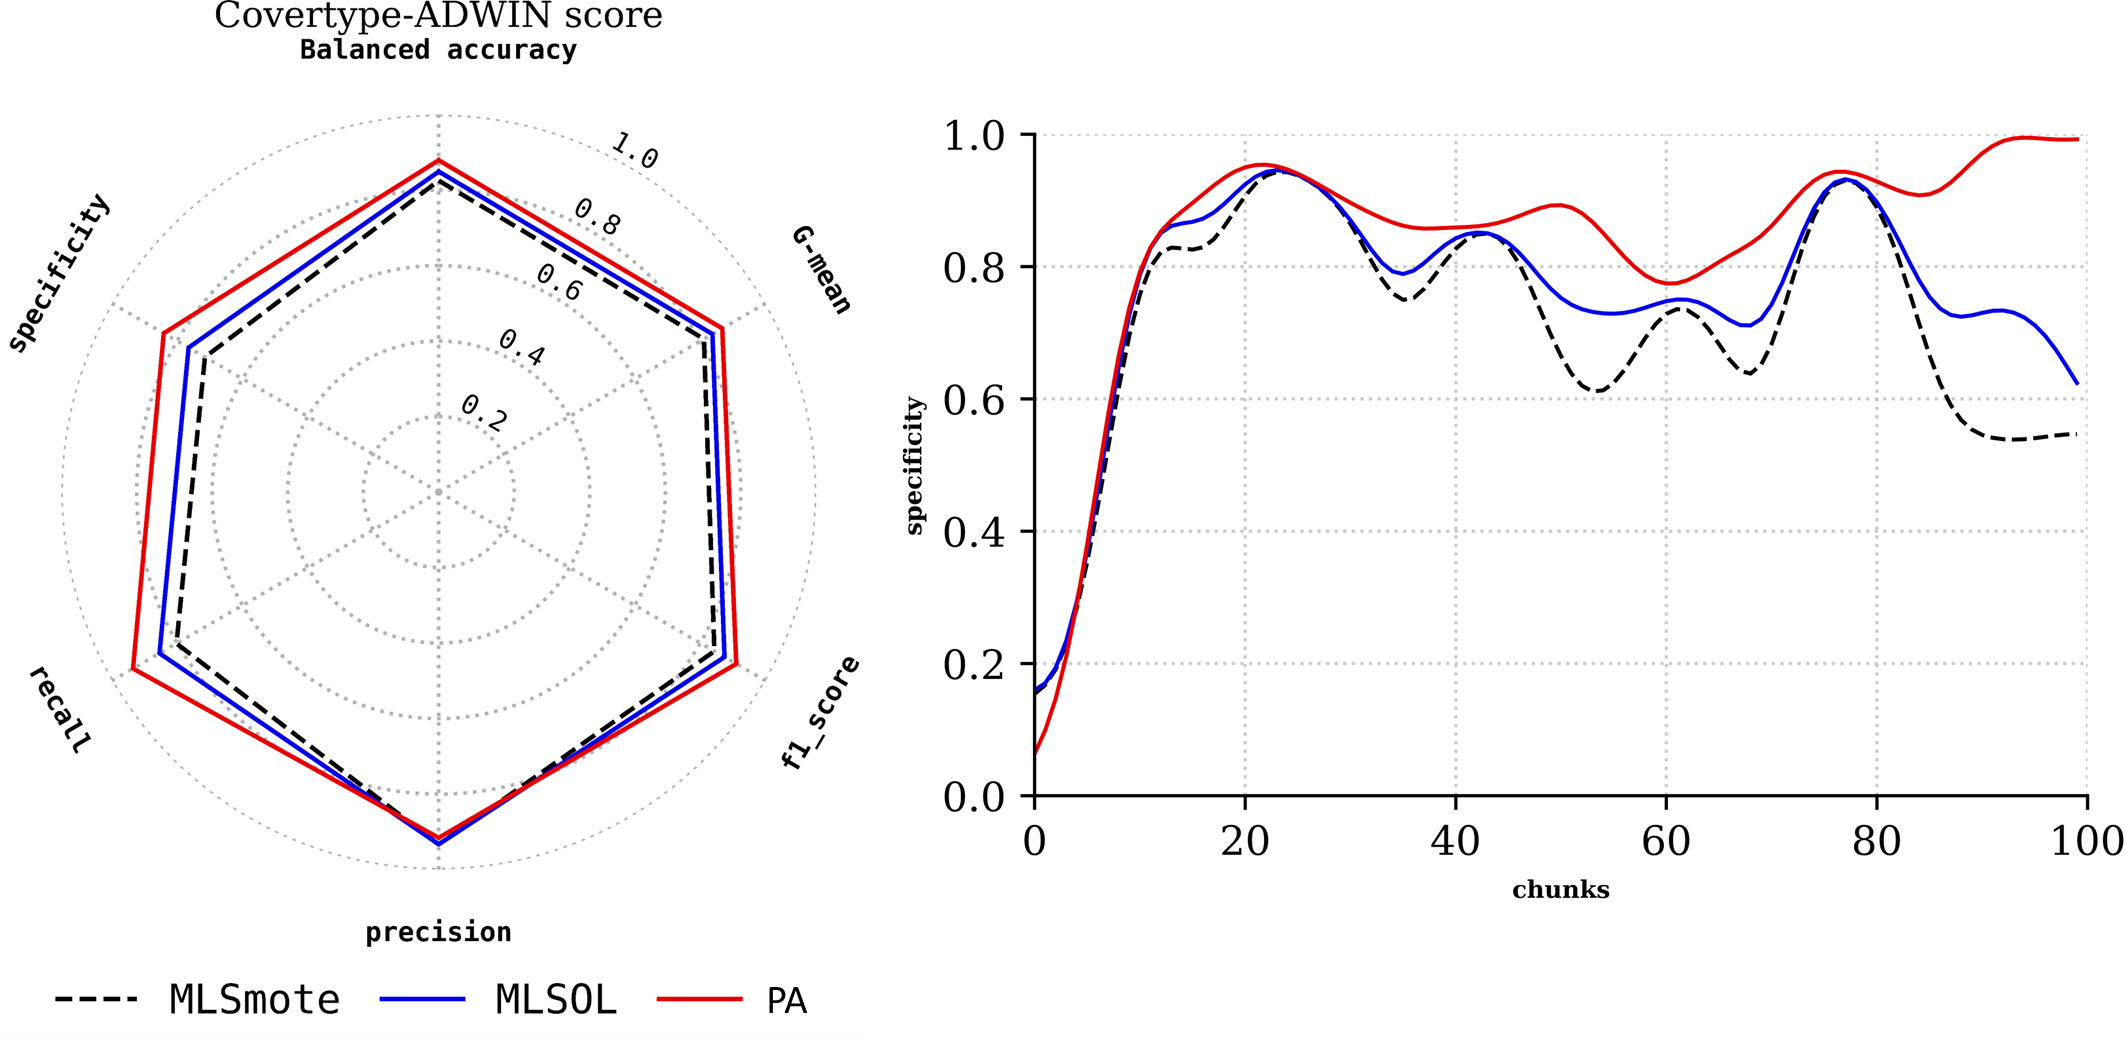
\includegraphics[width=1\linewidth]{4_Imbalanced/figures/exp_1.png}
	\caption{Comparison of PA1, MLSMOTE, and MLSOL on Covertype Dataset with ADWIN Concept Drift Detector.}
	\label{fig:4_first_proposal_result_exp_1}
\end{figure}
Figures \ref{fig:4_first_proposal_result_exp_1} and \ref{fig:4_first_proposal_result_exp_2} present the outcomes of applying MLSMOTE, MLSOL, and PA1 to the Covertype dataset, utilizing ADWIN and DDM as drift detectors, respectively.

In Fig. \ref{fig:4_first_proposal_result_exp_1}, the radar diagram provides a multidimensional perspective on the comparative performance of the three approaches across six critical metrics: precision, recall, specificity, F1 score, G-mean, and balanced accuracy. Each axis, normalized between 0 and 1, reveals the nuanced trade-offs inherent in these methods. PA1, denoted by the red line, consistently surpasses its counterparts in most metrics, particularly precision, F1 score, and G-mean, exemplifying its robustness in tackling the complexities of the Covertype dataset. MLSOL, represented by the blue line, exhibits a more balanced but less competitive performance, especially in specificity and G-mean. In contrast, MLSMOTE, illustrated by the dashed black line, demonstrates the least favorable performance, particularly struggling with recall and balanced accuracy. This visualization encapsulates the strengths and limitations of each approach, underscoring the philosophical interplay between metric optimization and algorithmic trade-offs in machine learning.

The line diagram within the same figure delves into the temporal evolution of classification accuracy, measured by specificity, over 100 data chunks. During the initial 20 chunks, all methods exhibit suboptimal performance, attributed to the nascent state of their classifier pools. This phase, marked by adaptation and learning, paves the way for a significant performance leap as the classifier pool expands. The Dynamic Ensemble Selection (DES) mechanism, empowered by this expansion, adeptly selects optimal classifiers for incoming data, driving a marked improvement in accuracy. Beyond chunk 20, PA1 emerges as the dominant performer, maintaining its supremacy throughout the subsequent chunks. Its superior performance stems from its strategic use of historical chunks to generate nonoverlapping and representative samples, which facilitate the effective training of pool classifiers. In contrast, MLSMOTE consistently lags behind, reflecting its limitations in leveraging the same adaptability.

Fig. \ref{fig:4_first_proposal_result_exp_2}, where DDM functions as the drift detector, offers a complementary perspective. The radar plot mirrors the relative performance hierarchy observed with ADWIN but with marginally diminished values across all metrics. The line diagram further corroborates PA1’s dominance, albeit with less pronounced gaps between the approaches. However, the overall reduction in performance across all methods highlights the comparative limitations of DDM in detecting and responding to concept drift within the Covertype dataset.

This juxtaposition of ADWIN and DDM as drift detectors underscores the profound impact of drift detection mechanisms on classifier performance. ADWIN’s demonstrated superiority in handling the intricate dynamics of the Covertype stream reaffirms its pivotal role in ensuring robust learning and adaptation. PA1’s sustained excellence across diverse scenarios, facilitated by its strategic use of historical knowledge and dynamic ensemble mechanisms, exemplifies a philosophical alignment between algorithmic design and the evolving nature of benchmark Stream data streams. These findings emphasize the necessity of harmonizing drift detection techniques with classifier methodologies to navigate the multifaceted challenges posed by non-stationary environments, thereby advancing the frontiers of machine learning research.

\vspace{-2mm}
\begin{figure}[H]
	\centering
	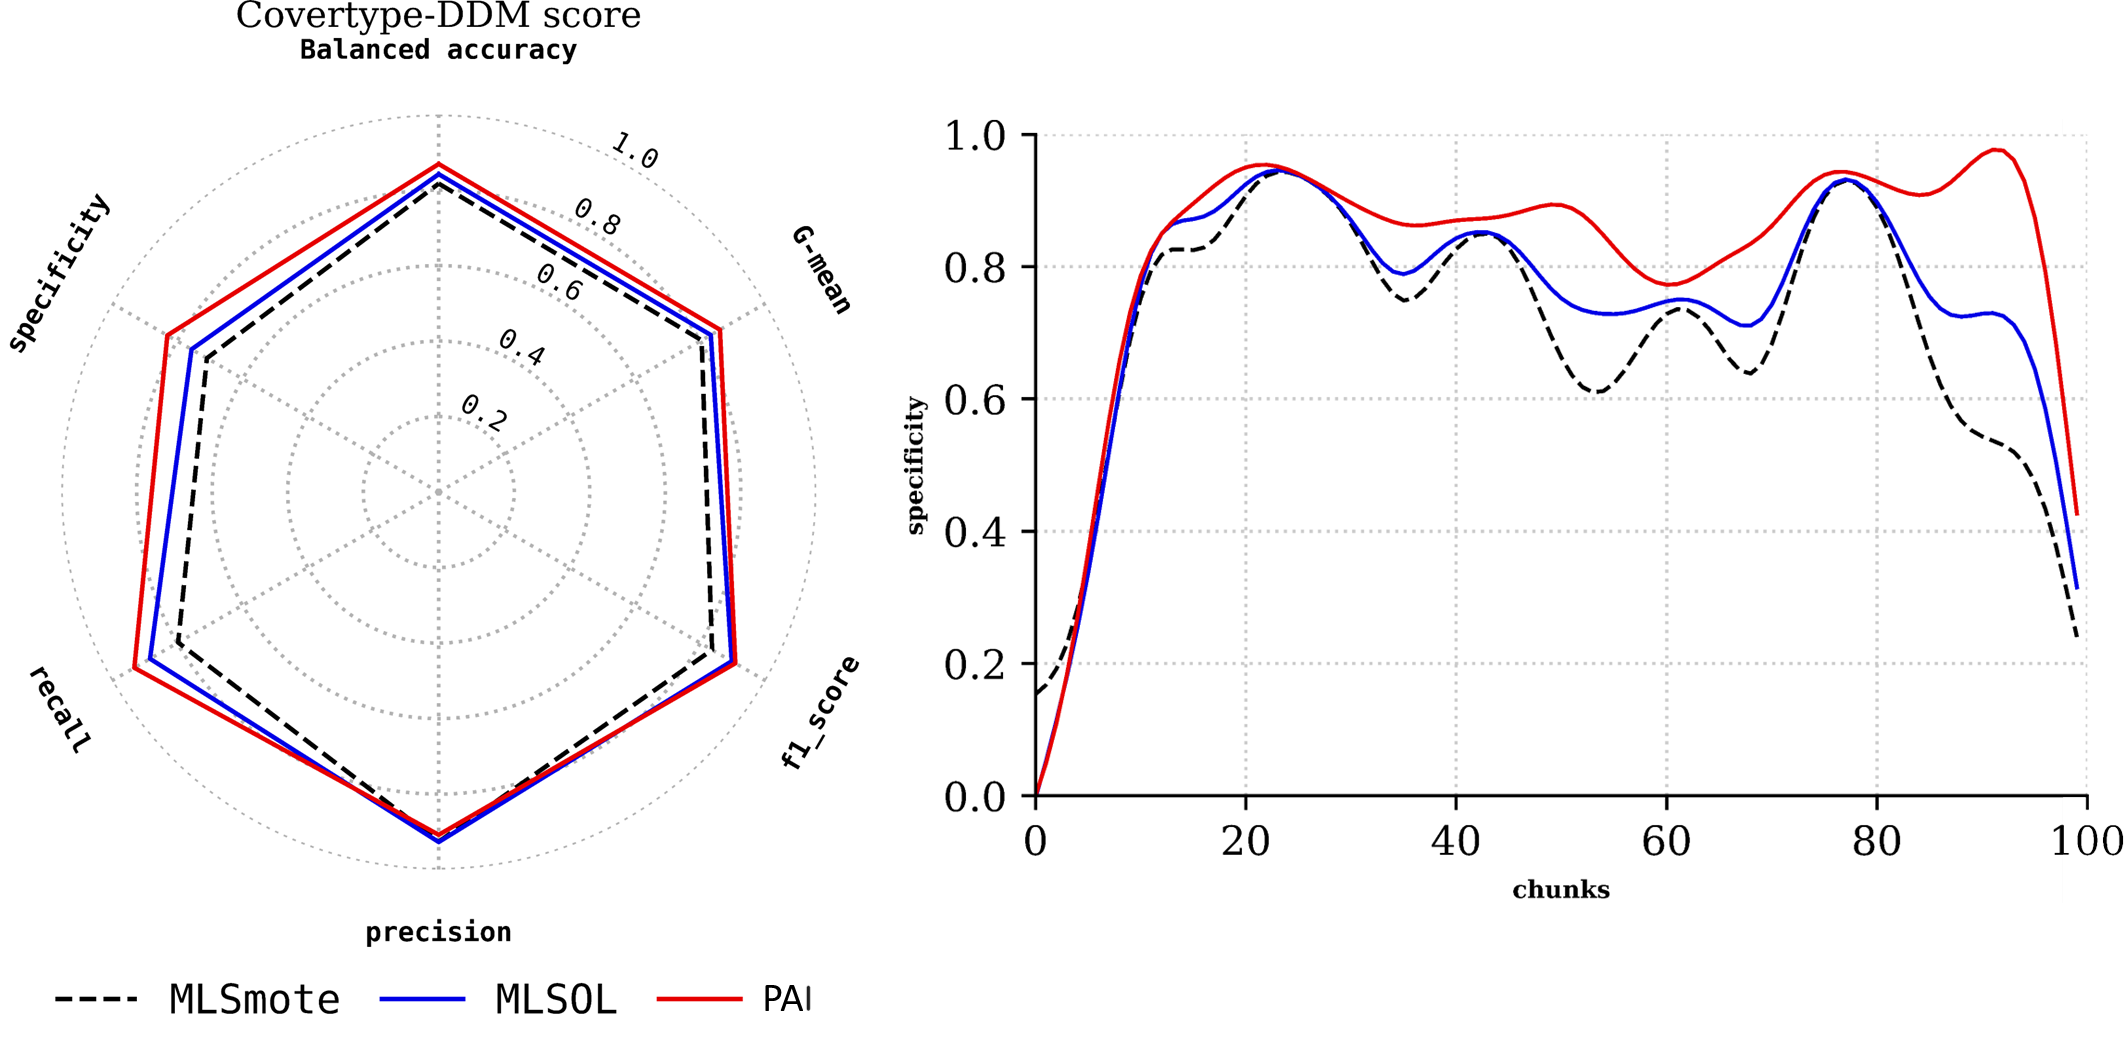
\includegraphics[width=1\linewidth]{4_Imbalanced/figures/exp_2.png}
  \caption{Comparison of PA1, MLSMOTE, and MLSOL on Covertype Dataset with DDM Concept Drift Detector.}
	\label{fig:4_first_proposal_result_exp_2}
\end{figure}

\subsubsection{Results on the Real Application Stream}
Figures \ref{fig:4_first_proposal_result_exp_3} and \ref{fig:4_first_proposal_result_exp_4} demonstrate the performance of the three evaluated methods—PA1, MLSMOTE, and MLSOL—on the Sensor data stream using ADWIN and DDM as drift detectors, respectively.

In Fig. \ref{fig:4_first_proposal_result_exp_3}, the radar plot reveals metric values primarily between 0.6 and 0.8, underscoring the inherent drift and imbalance present in the Sensor stream. While precision and recall metrics for all three methods appear nearly identical, PA1 exhibits a pronounced advantage across the remaining metrics. The similarity in performance between MLSMOTE and MLSOL reflects their comparable strategies in handling imbalanced streams, yet neither matches PA1's robustness.

The line plot provides deeper insight into the temporal dynamics of the methods. During the initial 30 chunks, PA1 demonstrates a transient suboptimal phase, likely due to its limited pool of classifiers. However, as the pool expands over time, PA1's performance improves significantly, achieving consistent superiority across subsequent chunks. MLSMOTE and MLSOL, in contrast, display fluctuations, with each excelling in alternate chunks but failing to maintain consistent performance. These observations highlight PA1's ability to adapt and sustain its performance in the face of continuous challenges.

Fig. \ref{fig:4_first_proposal_result_exp_4} shifts the perspective to DDM as the drift detector. While the radar plot indicates a general decline in metric values compared to the ADWIN-based results, the line plot reaffirms PA1's dominance across most chunks. Nevertheless, the overall convergence of method performance over time, coupled with the reduced effectiveness of all approaches under DDM, underscores the sensitivity of drift detection mechanisms to data characteristics.

The comparative analysis between Figures \ref{fig:4_first_proposal_result_exp_3} and \ref{fig:4_first_proposal_result_exp_4} emphasizes ADWIN's superiority over DDM when applied to the Sensor data stream. This distinction reveals the intricate interplay between drift detection and classifier performance, affirming the pivotal role of appropriate drift detection mechanisms in achieving optimal outcomes. PA1’s consistent adaptability and resilience, regardless of the underlying drift detector, further solidify its potential as a robust solution in addressing complex, non-stationary, and imbalanced data streams. These findings not only highlight the efficacy of PA1 but also underscore the necessity of harmonizing algorithm design with drift detection strategies to address the multifaceted challenges posed by real-world data streams.
 
\begin{figure}[!ht]
	\centering
	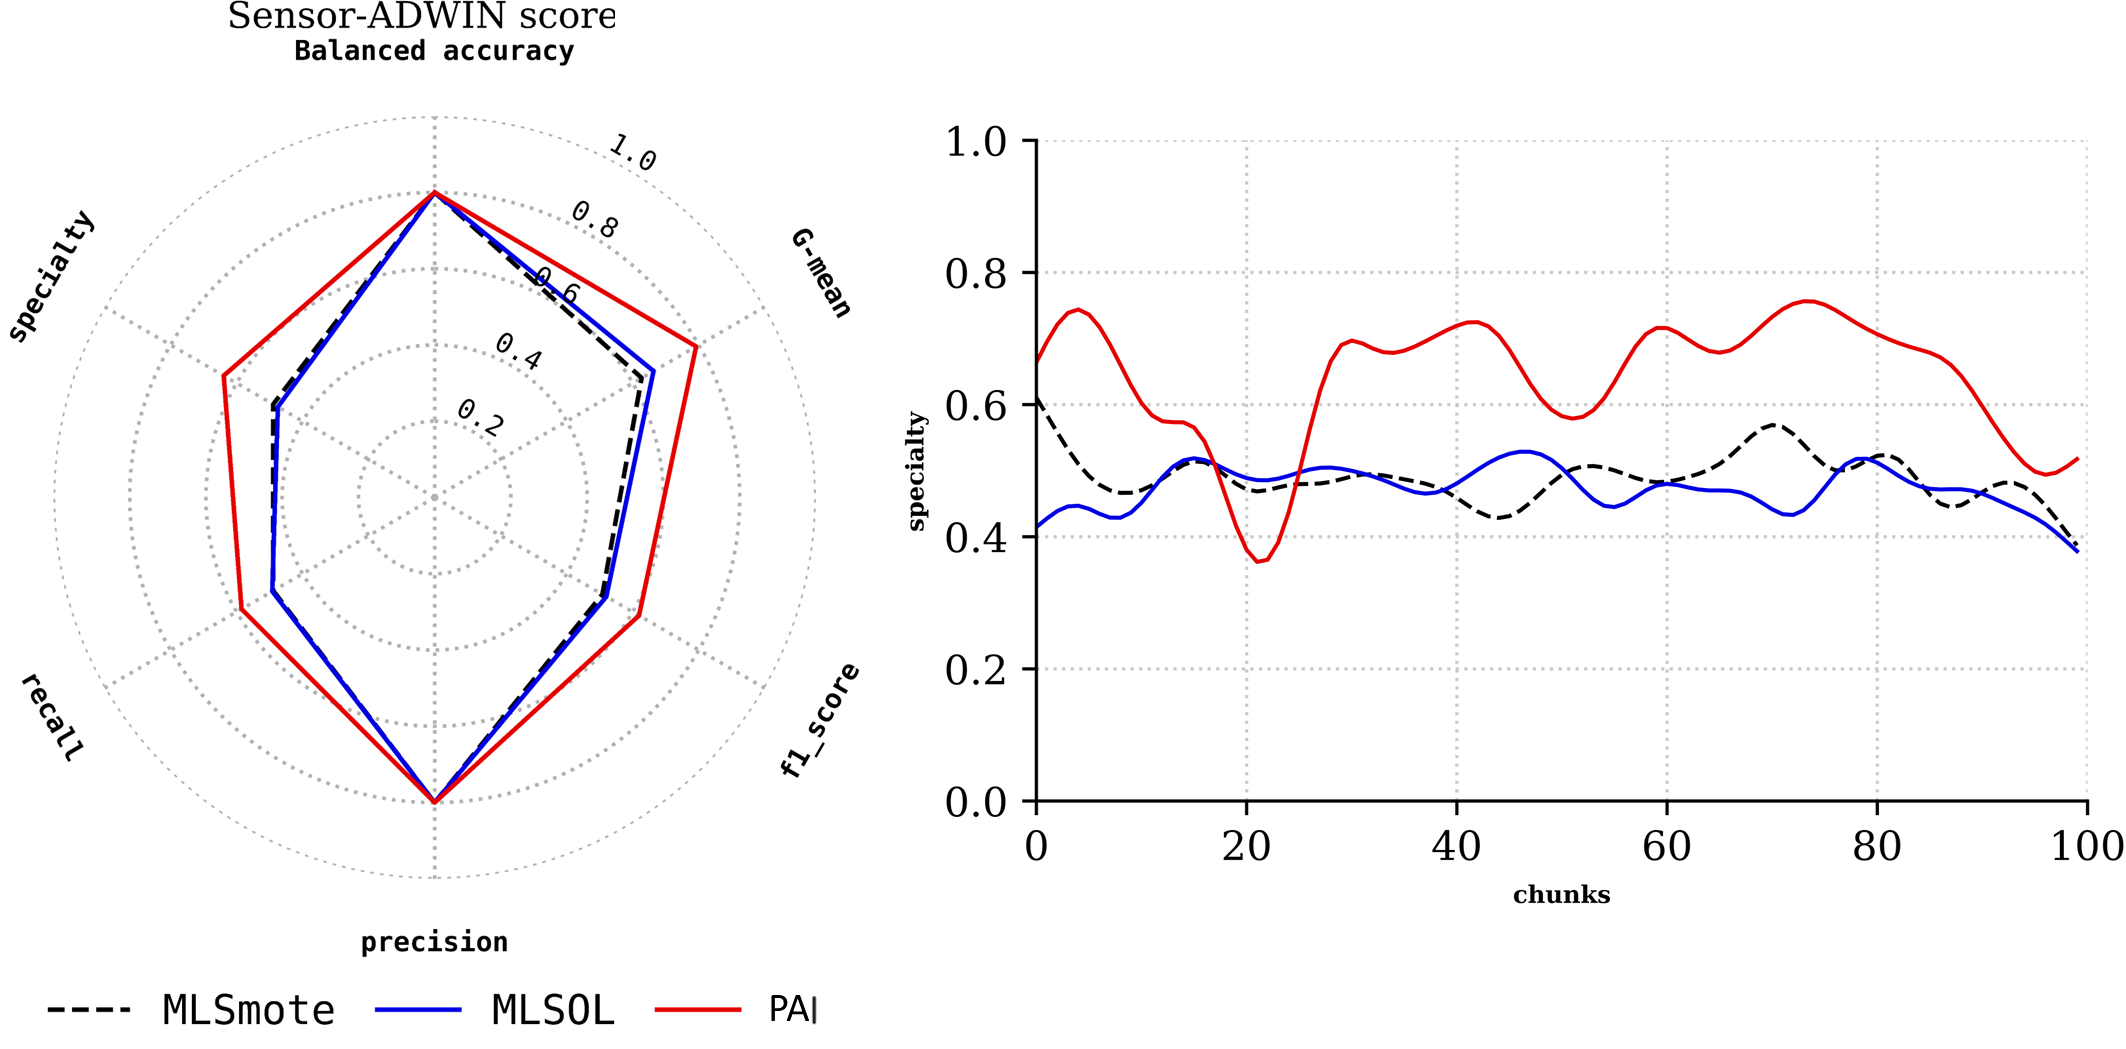
\includegraphics[width=1\linewidth]{4_Imbalanced/figures/exp_3.png}
  \caption{Comparison of PA1, MLSMOTE, and MLSOL on Sensor Dataset with ADWIN Concept Drift Detector.}
	\label{fig:4_first_proposal_result_exp_3}
\end{figure}

\begin{figure}[!ht]
	\centering
	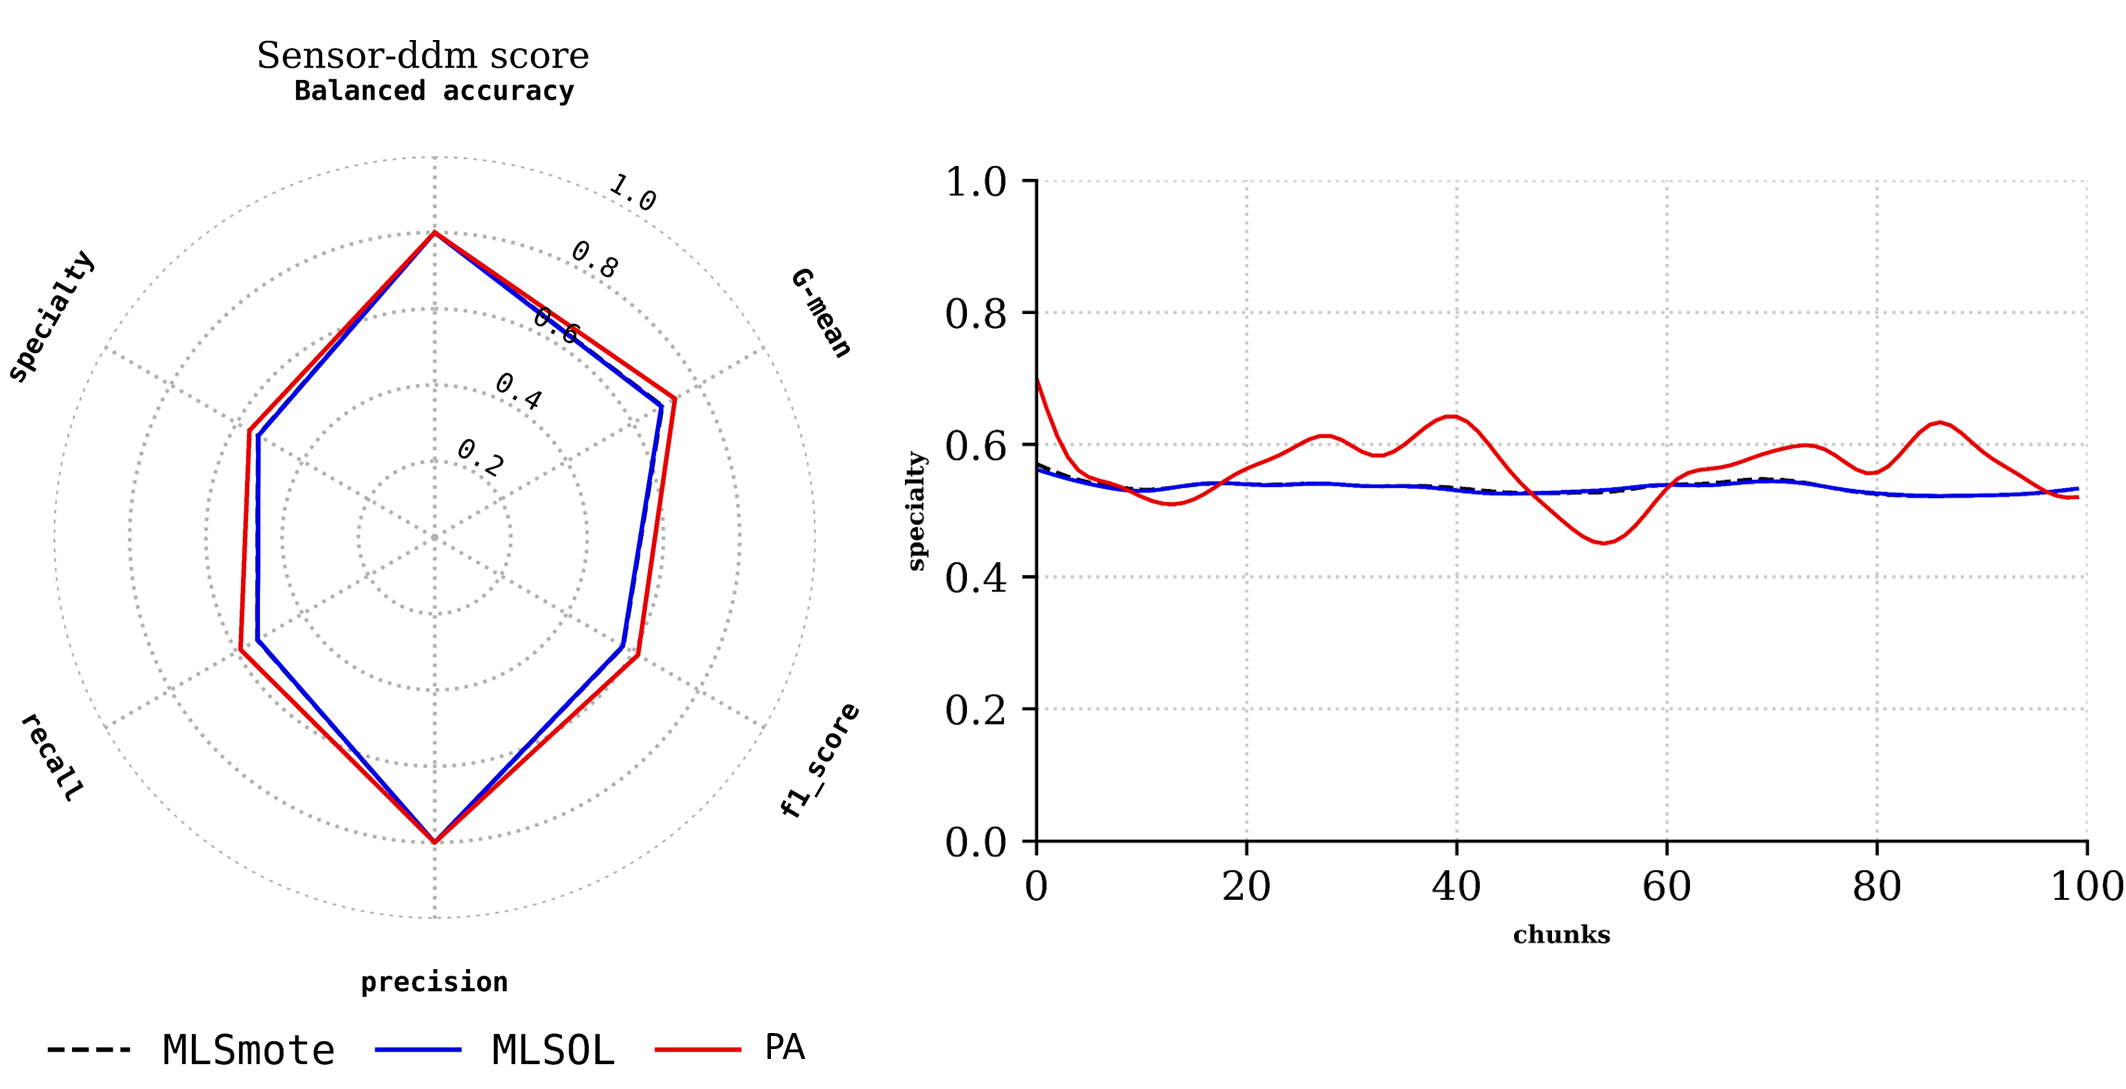
\includegraphics[width=1\linewidth]{4_Imbalanced/figures/exp_4.png}
  \caption{Comparison of PA1, MLSMOTE, and MLSOL on Sensor Dataset with DDM Concept Drift Detector}.
	\label{fig:4_first_proposal_result_exp_4}
\end{figure}

\subsubsection{Results on the Synthetic Stream}

Figures \ref{fig:4_first_proposal_result_exp_5} and \ref{fig:4_first_proposal_result_exp_6} illustrate the performance of the evaluated methods on the synthetic data stream using ADWIN and DDM as concept drift detectors, respectively.

In Fig. \ref{fig:4_first_proposal_result_exp_5}, the radar plot reflects metric values predominantly ranging between 0.6 and 0.8, highlighting the susceptibility of the synthetic stream to frequent drifts. The methods demonstrate divergent capabilities: MLSOL achieves the highest precision, while MLSMOTE records the lowest performance across metrics. Notably, PA1 emerges as the superior approach in metrics other than precision, showcasing its robustness in the presence of frequent drifts. The accompanying line plot underscores a transitional phase in PA1’s performance during the initial ten chunks, which can be attributed to the limited size of its classifier pool. However, beyond this initial phase, PA1 exhibits a significant and sustained improvement, consistently outperforming MLSOL and MLSMOTE across subsequent chunks. These results underscore the adaptability and effectiveness of PA1 in dynamically adjusting to the evolving data stream.

Fig. \ref{fig:4_first_proposal_result_exp_6} reveals analogous patterns when employing DDM as the drift detector. The radar plot metrics align with those observed in the previous experiment, reinforcing the insights gleaned from ADWIN-based evaluation. However, the line diagram highlights a subtle degradation in the performance of MLSOL and MLSMOTE compared to the ADWIN experiment. This variation underscores the sensitivity of these techniques to the underlying drift detection mechanism. PA1, in contrast, maintains its consistent superiority, further validating its robustness and adaptability across diverse drift detectors.

The comparative analysis of ADWIN and DDM affirms the superiority of ADWIN in handling synthetic data streams, where abrupt and frequent concept drifts pose substantial challenges. These findings transcend the experimental domain, illustrating the versatility and resilience of PA1 in addressing concept drift across diverse datasets, including the synthetic, Covertype, and Sensor datasets. This robustness, coupled with its adaptability to different drift detection mechanisms, reflects the algorithm's capacity to harmonize precision with recall, even under challenging conditions. Thus, PA1 emerges as a paradigm of effective learning in the non-stationary realm, embodying the intricate interplay between adaptability, precision, and robustness essential for real-world applications.

\begin{figure}[!ht]
	\centering
	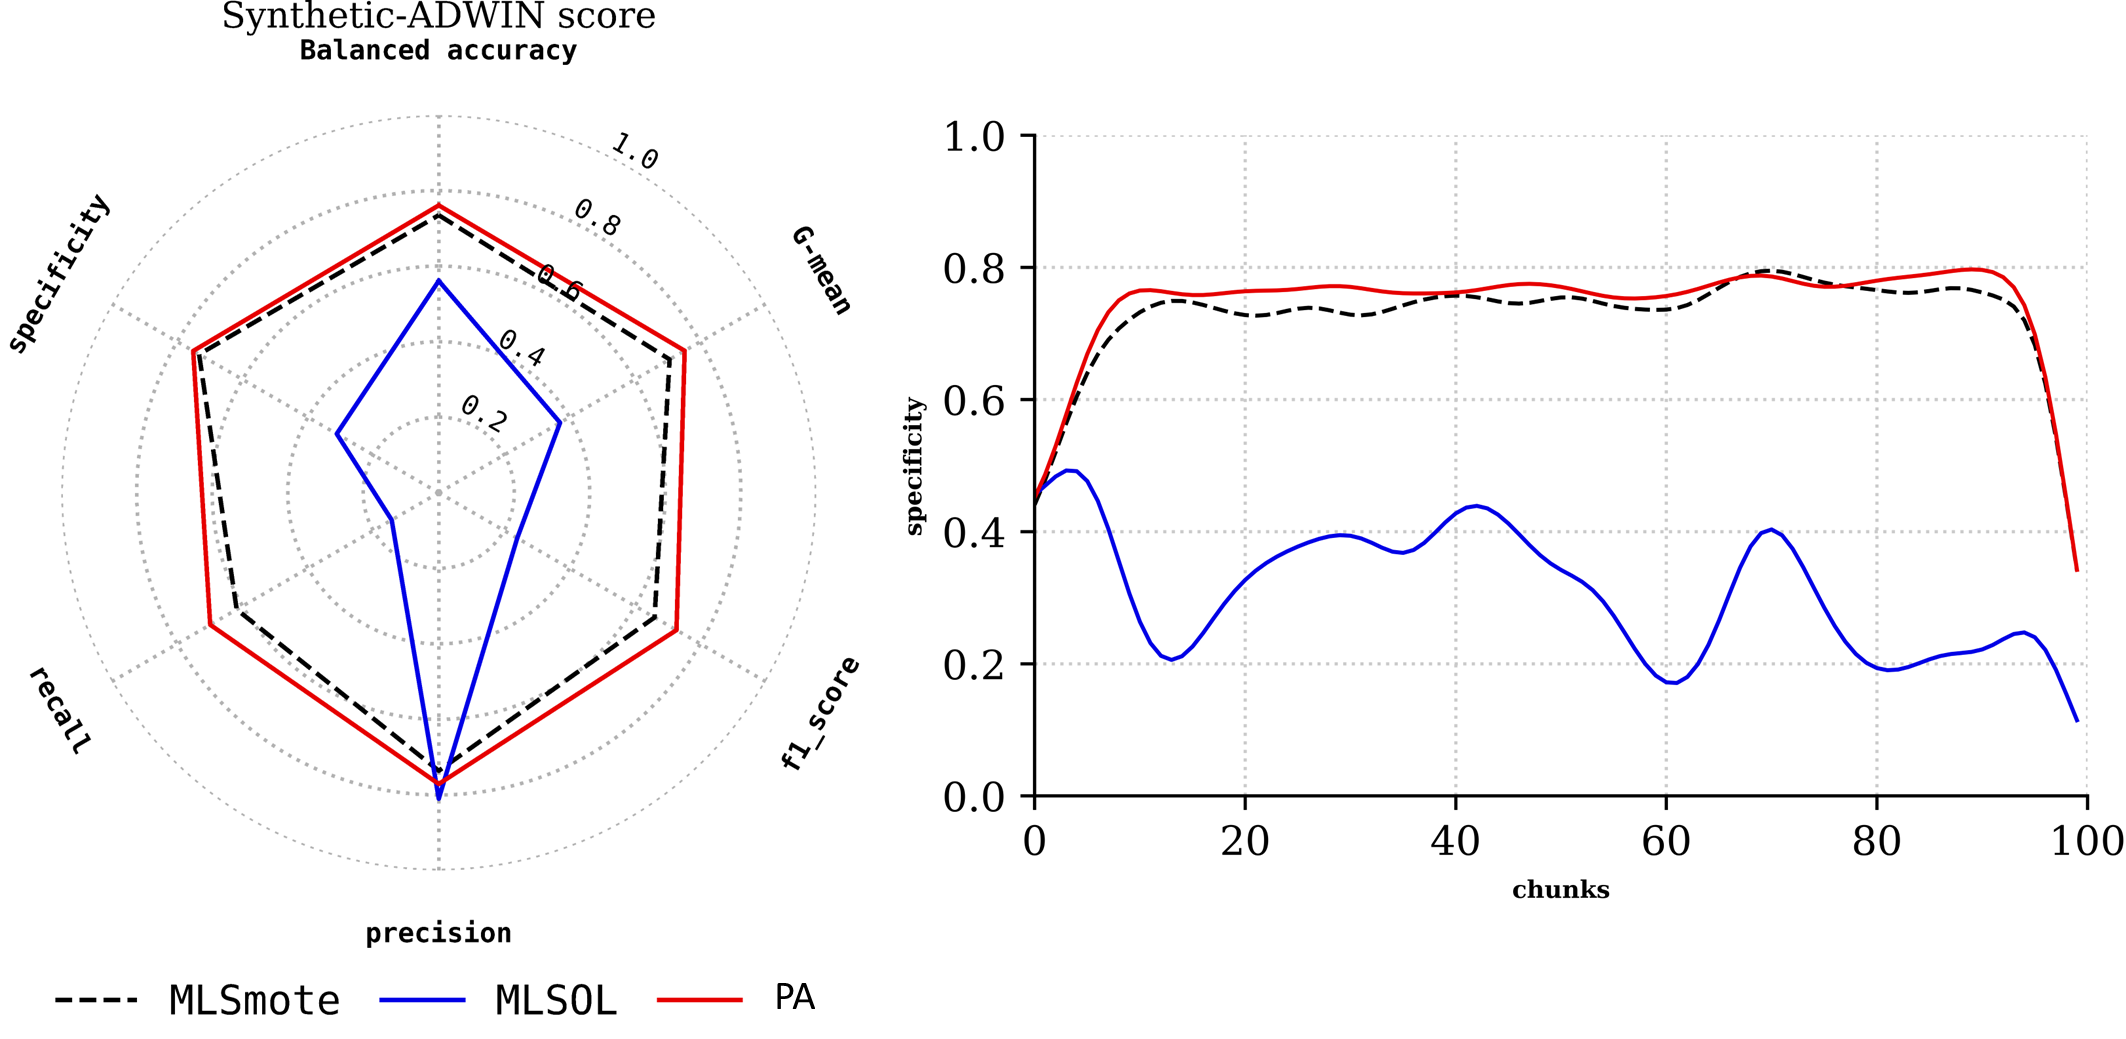
\includegraphics[width=1\linewidth]{4_Imbalanced/figures/exp_5.png}
  \caption{Comparison of PA1, MLSMOTE, and MLSOL on Synthetic Dataset with ADWIN Concept Drift Detector.}
	\label{fig:4_first_proposal_result_exp_5}
\end{figure}

\begin{figure}[!ht]
	\centering
	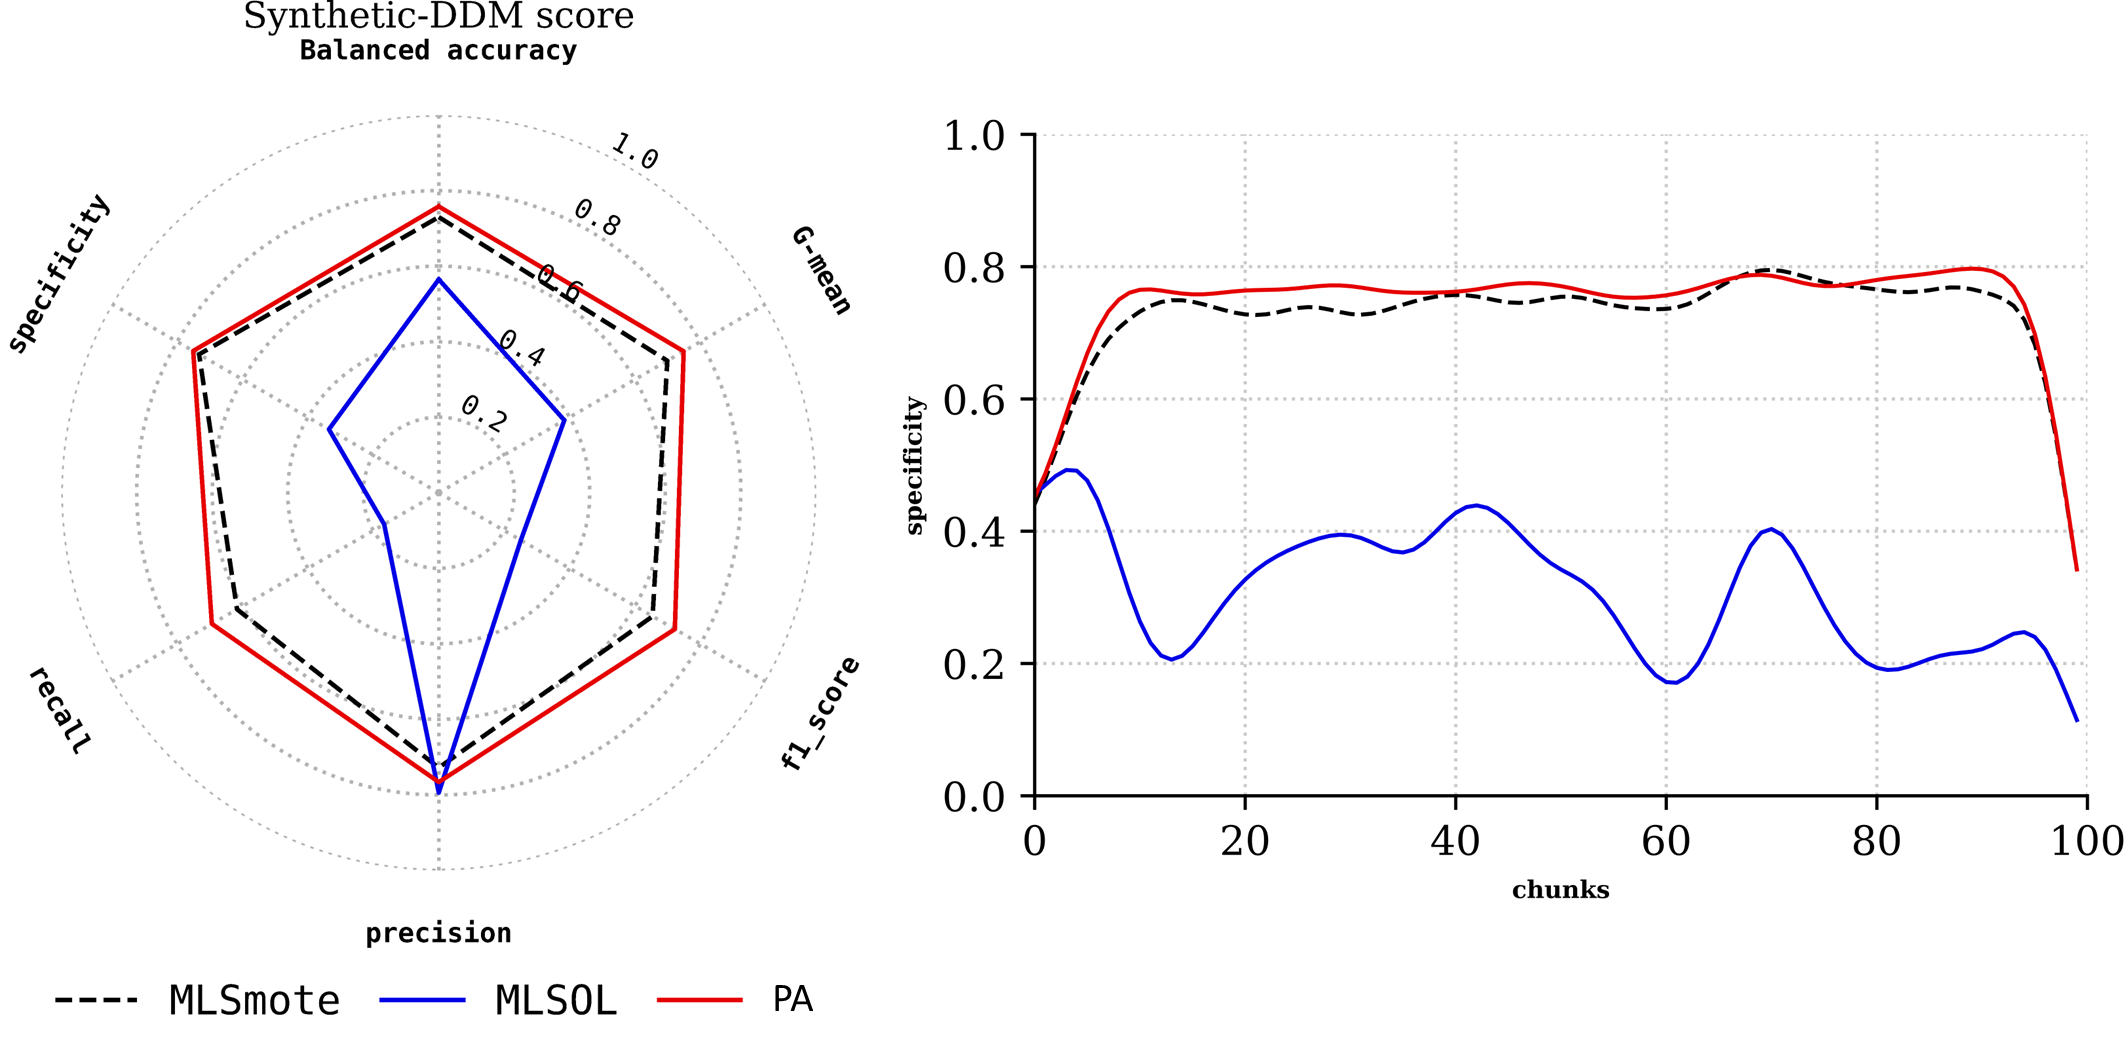
\includegraphics[width=1\linewidth]{4_Imbalanced/figures/exp_6.png}
  \caption{Comparison of PA1, MLSMOTE, and MLSOL on Synthetic Dataset with DDM Concept Drift Detector.}
	\label{fig:4_first_proposal_result_exp_6}
\end{figure}


\subsection{Analysis of Class Overlap Factor between Proposed Approach (PA1), MLSMOTE, and MLSOL Techniques.}
In our experimental study, we aimed to identify the critical factors that influence the selection of an optimal approach for minority classes in imbalanced drifted streams. These factors include various aspects, such as dataset characteristics, the choice of concept drift detectors, and the effectiveness of the algorithm in handling class overlap. To compare the overlapping class behavior of first proposed approach (PA1) with MLSMOTE and MLSOL, we systematically designed experiments organized into groups of ten chunks. The results were visualized in bar diagrams, contrasting PA1 with other methods (MLSMOTE and MLSOL). Figures \ref{fig:4_first_proposal_result_exp_7}\ref{fig:4_first_proposal_result_exp_8}\ref{fig:4_first_proposal_result_exp_9} present ten groups, each with three bars representing MLSOTE, MLSOL, and PA1, respectively. Each bar visually represents overlapped samples for ten chunks of several data streams, considering distinct concept drift detectors, specifically ADWIN and DDM.
Fig. \ref{fig:4_first_proposal_result_exp_7} shows two diagrams for the ADWIN and DDM detectors. In the ADWIN diagram, the third bar group (chunks 20-30) lacks overlapping samples because this chunk range does not have drifts, and no synthetic samples are generated for the training step. The sixth and tenth groups have the highest overlapped samples because these groups experience many drifts, leading to the generation of several samples and, consequently, the data indicates that MLSMOTE displays the highest number of overlapping samples across all groups, while PA1 exhibits very few, except for the last group (90-100), which has a small number of overlapping samples. However, the DDM diagram has more overlapping samples than the ADWIN diagram because the DDM detector detects fewer drifts than ADWIN. Specifically, the last value on the Y-axis of the ADWIN diagram is 3,000 samples, while the last value on the Y-axis of the DDM diagram is 2,000 samples. Fig. \ref{fig:4_first_proposal_result_exp_8} and Fig. \ref{fig:4_first_proposal_result_exp_9} display the overlapping samples of the three methods on the Sensor and synthetic data streams, respectively. In Fig. \ref{fig:4_first_proposal_result_exp_8}, the ADWIN diagram demonstrates fewer overlapped samples than in Fig. \ref{fig:4_first_proposal_result_exp_8}, indicating a lower number of drifts in the Sensor stream. The overall diagram indicates that first proposed approach achieves fewer overlapped samples than MLSOL and MLSMOTE, with MLSMOTE having the highest number of overlapped samples. In the DDM diagram of Fig. 10, the number of overlapped samples is lower than in Fig. \ref{fig:4_first_proposal_result_exp_7}, with first proposed approach consistently achieving the lowest number of overlapped samples across most group bars.
In Fig. \ref{fig:4_first_proposal_result_exp_9}, the ADWIN and DDM diagrams exhibit the greatest number of overlapped samples compared to the earlier figures. This suggests that the synthetic stream underwent frequent drifts and was more susceptible to noise. Consequently, the last value on the Y-axis in both the ADWIN and DDM diagrams was recorded for 7,000 samples. First proposed approach consistently achieves the lowest number of overlapped samples, whereas MLSMOTE consistently attains the highest number of overlapped samples across most group bars in both the ADWIN and DDM diagrams. In conclusion, our thorough examination of overlapping class instances across MLSMOTE, MLSOL, and first approach consistently reveals minimal overlapped samples compared to other methods, regardless of whether DDM or ADWIN is employed as drift detectors

\begin{figure}[!ht]
	\centering
	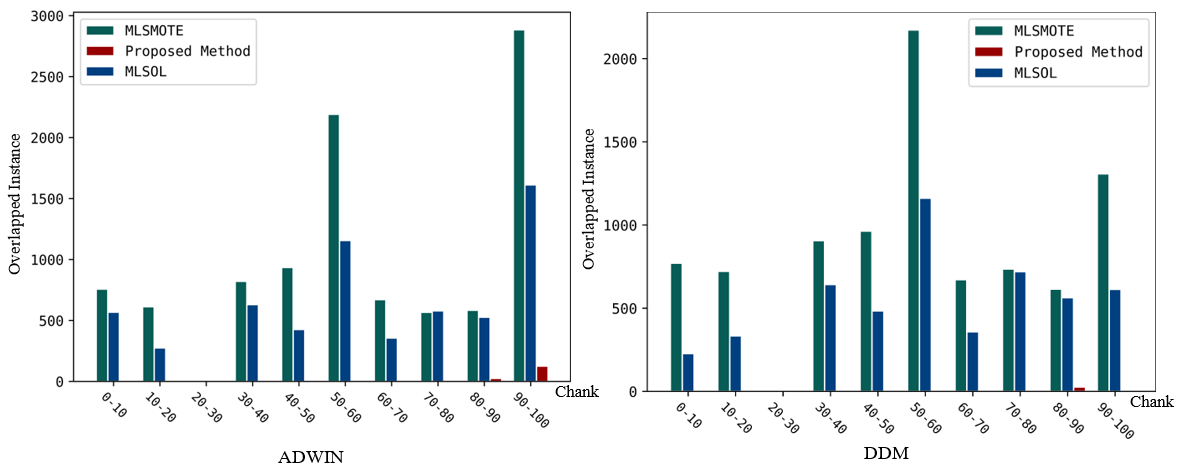
\includegraphics[width=1\linewidth]{4_Imbalanced/figures/exp_7.png}
  \caption{Overlapping Points of PA1, MLSMOTE, and MLSOL on Covertype Stream.}
	\label{fig:4_first_proposal_result_exp_7}
\end{figure}

\begin{figure}[!ht]
	\centering
	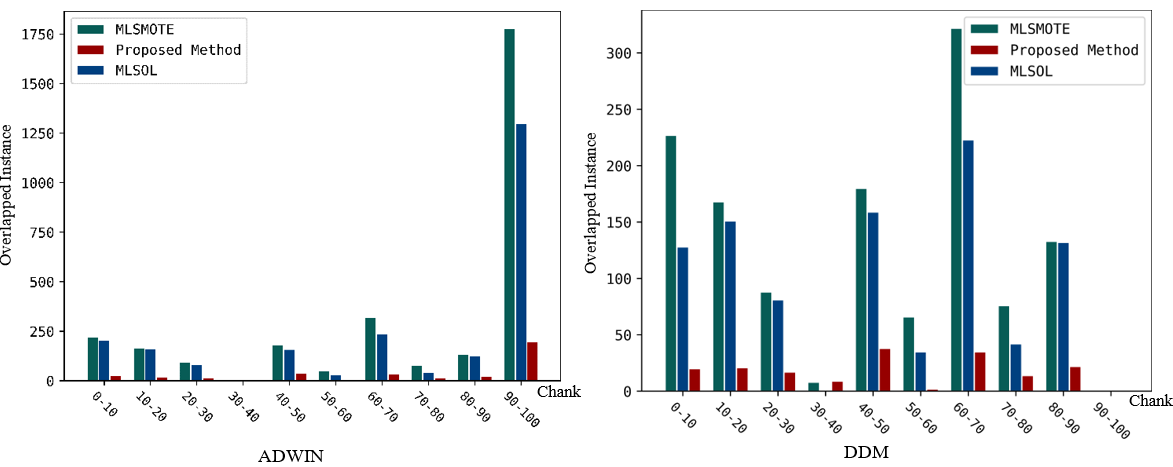
\includegraphics[width=1\linewidth]{4_Imbalanced/figures/exp_8.png}
  \caption{Overlapping Points of PA1, MLSMOTE, and MLSOL on Sensor Stream.}
	\label{fig:4_first_proposal_result_exp_8}
\end{figure}

\begin{figure}[!ht]
	\centering
	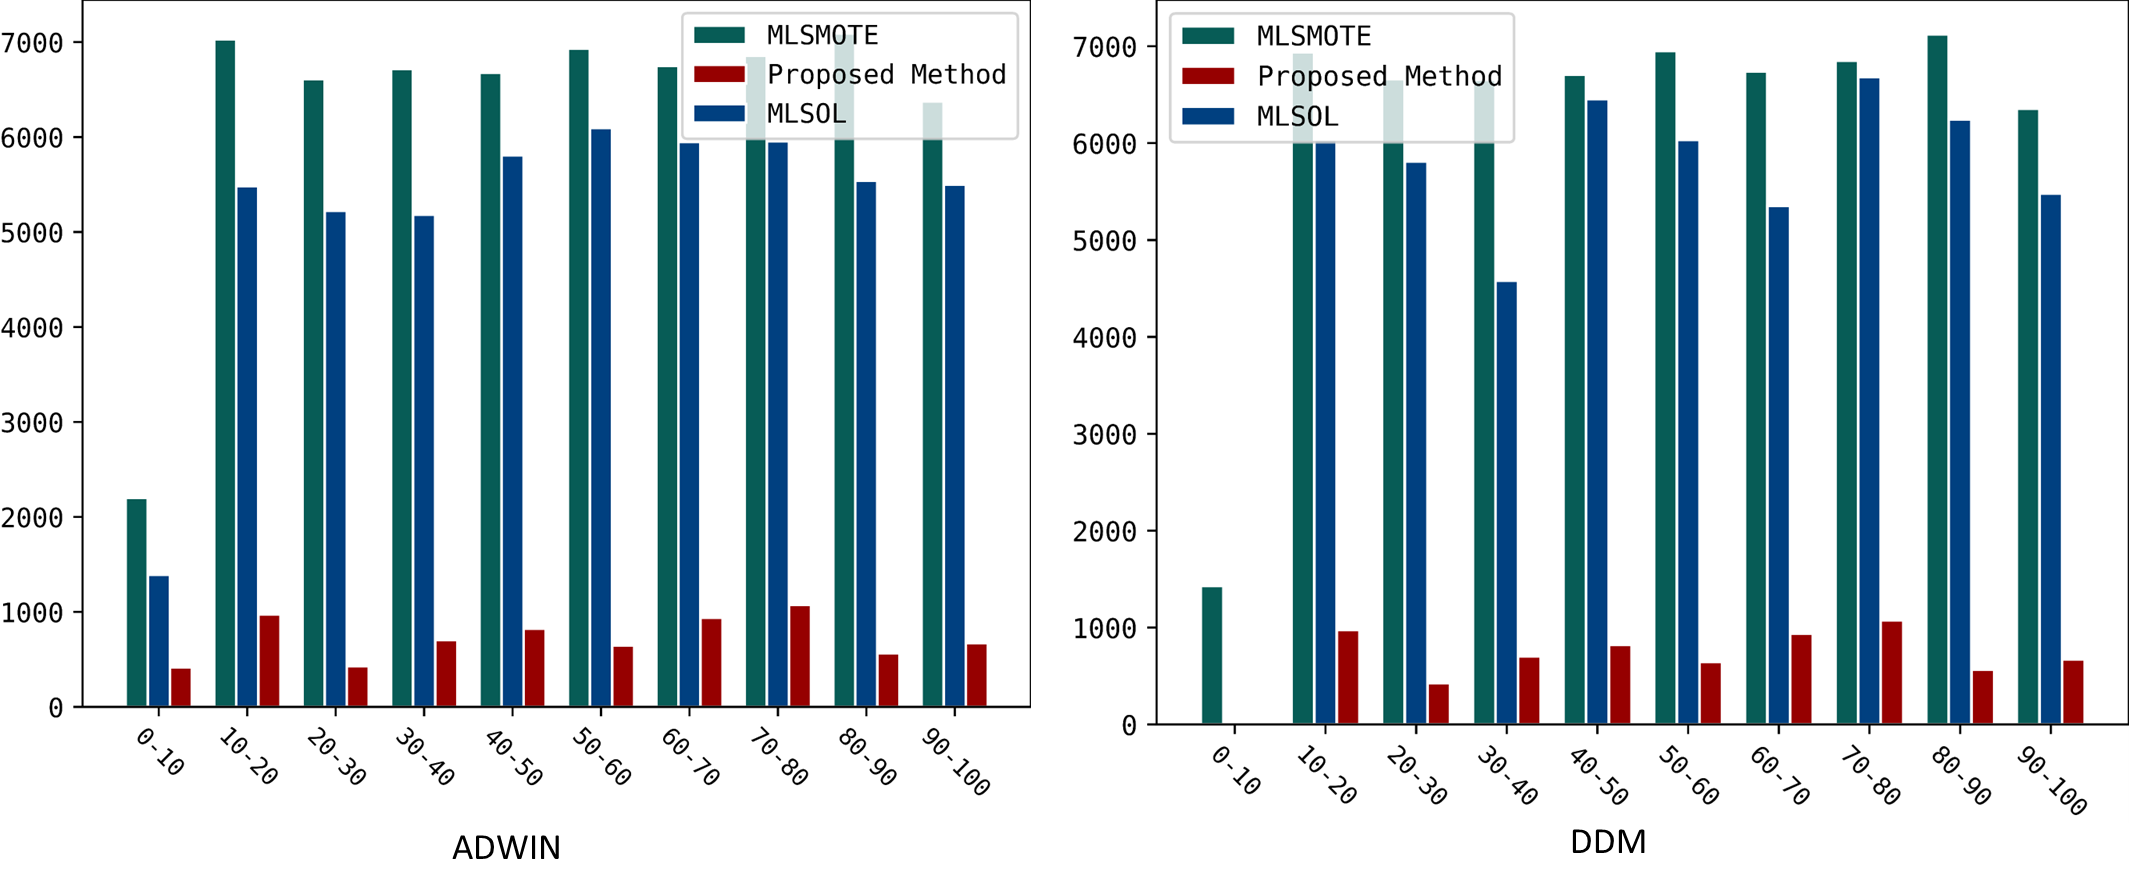
\includegraphics[width=1\linewidth]{4_Imbalanced/figures/exp_9.png}
  \caption{Overlapping Points of PA1, MLSMOTE, and MLSOL on Synthetic Stream.}
	\label{fig:4_first_proposal_result_exp_9}
\end{figure}

\subsection{Analyzing Runtime Factor Between the First Proposed Approach, MLSMOTE, and MLSOL Techniques}
The results of our experiments indicate that the choice of the best algorithm for multiclass imbalanced streams depends on various factors, including dataset characteristics, the concept drift detector used, the presence of an overlapping class problem, and the algorithm's runtime demands. To investigate the runtimes of MLSMOTE, MLSOL, and first approach, we conducted experiments, as shown in Table \ref{tab:4_first_proposal_result_table_2}. Our findings reveal that first proposed approach is highly efficient, regardless of whether ADWIN or DDM is used as the concept drift detector. Specifically, when ADWIN was used, the first proposed approach algorithm took 8344 s to train and predict the Covertype stream for ensemble classifiers, whereas it took 8019 s when using the DDM detector. In contrast, MLSMOTE and MLSOL require more time for the same task. Notably, first approach maintains efficiency, even when using the DDM concept detector. Additionally, first approach demonstrates shorter processing times in the Sensor stream and synthetic data compared with other methods. Consistently, the DDM detector achieved less time across all experiments owing to its lower detection of drifts compared to the ADWIN detector. This is because there are fewer instances that trigger training for pool classifiers when using the DDM. The bold highlighting in Table \ref{tab:4_first_proposal_result_table_2} further emphasizes the efficiency of first approach with both the ADWIN and DDM detectors across all dataset streams. Because our proposal generates fewer overlapped samples, leading to an overall decrease in the running time.

\begin{table}[h!]
  \centering
  \caption{Runtimes (in seconds) Comparison of PA1, MLSMOTE, and MLSOL.}
  \resizebox{\textwidth}{!}{
  \begin{tabular}{|l|l|c|c|c|}
  \hline
  \textbf{Stream} & \textbf{Concept Drift Detector} & \textbf{MLSMSOTE} & \textbf{MLSOL} & \textbf{PA1} \\ \hline
  \multirow{2}{*}{Benchmark} & ADWIN & 9559 & 8655 & \textbf{8344} \\ \cline{2-5} 
   & DDM & 8388 & 8031 & \textbf{8019} \\ \hline
  \multirow{2}{*}{Real Application} & ADWIN & 1291 & 1310 & \textbf{1102} \\ \cline{2-5} 
   & DDM & 585 & 607 & \textbf{521} \\ \hline
  \multirow{2}{*}{Synthetic} & ADWIN & 12870 & 4866 & \textbf{4834} \\ \cline{2-5} 
   & DDM & 12397 & 4958 & \textbf{4687} \\ \hline
  \end{tabular}
  }
  \label{tab:4_first_proposal_result_table_2}
  \end{table}

\subsection{Analyzing Non-parametric Tests between the First Proposed Approach, MLSMOTE, and MLSOL Techniques}
We conducted a thorough series of statistical analyses encompassing 12 comparisons across three diverse datasets, three methods, and two drift detectors. These analyses were rigorously evaluated using a non-parametric test, specifically the Kruskal-Wallis test. The results of this test were striking, revealing substantial variations in the G-mean measurements across most experiments. Importantly, these differences were not due to random chance \cite{yamada2013change}. Upon closer examination of the assessments for the three methods, PA1, MLSMOTE, and MLSOTE, as detailed in Table \ref{tab:4_first_proposal_result_table_3}, we found compelling evidence supporting the acceptance of the null hypothesis (H0).
This implies that the expected and observed data exhibited statistically significant disparities. H0 is rejected when significant differences are not observed and H0 is accepted if the P-value falls below the critical value. Underlining the significance of our analysis, the Kruskal-Wallis test was conducted with a 95\% confidence level, and the P-value was rounded to the first three digits after the decimal point. Nevertheless, it is important to note that a similarity in the performances of the methods emerged in the third and fourth experiments, resulting in the rejection of H0. This similarity can be attributed to the fact that the DDM detected fewer drifts in these experiments.


\begin{table}[h!]
  \centering
  \caption{Kruskal-Wallis test results for MLSMOTE, MLSOL, and PA1.}
  \resizebox{\textwidth}{!}{
  \begin{tabular}{|c|c|c|c|c|c|}
  \hline
  \multirow{2}{*}{Dataset} & \multirow{2}{*}{Drift detector} & \multirow{2}{*}{Comparison} & \multirow{2}{*}{P-value} & \multirow{2}{*}{Critical value} & \multirow{2}{*}{H0} \\ 
                           &                                 &                             &                           &                                 &  \\
  \hline
  \multirow{4}{*}{Covertype stream} & \multirow{2}{*}{ADWIN} & PA1 - MLSSMOTE & 0.001 & 0.05 & Accept \\ \cline{3-6}
                                    &                        & PA1 - MLSOL    & 0.014 & 0.05 & Accept \\ \cline{2-6}
                                    & \multirow{2}{*}{DDM}   & PA1 - MLSSMOTE & 0.361 & 0.05 & Rejected \\ \cline{3-6}
                                    &                        & PA1 - MLSOL    & 0.401 & 0.05 & Rejected \\ 
  \hline
  \multirow{4}{*}{Sensor stream} & \multirow{2}{*}{ADWIN} & PA1 - MLSSMOTE & 0.001 & 0.05 & Accept \\ \cline{3-6}
                                 &                        & PA1 - MLSOL    & 0.001 & 0.05 & Accept \\ \cline{2-6}
                                 & \multirow{2}{*}{DDM}   & PA1 - MLSSMOTE & 0.001 & 0.05 & Accept \\ \cline{3-6}
                                 &                        & PA1 - MLSOL    & 0.001 & 0.05 & Accept \\ 
  \hline
  \multirow{4}{*}{Synthetic stream} & \multirow{2}{*}{ADWIN} & PA1 - MLSSMOTE & 0.001 & 0.05 & Accept \\ \cline{3-6}
                                    &                        & PA1 - MLSOL    & 0.001 & 0.05 & Accept \\ \cline{2-6}
                                    & \multirow{2}{*}{DDM}   & PA1 - MLSSMOTE & 0.001 & 0.05 & Accept \\ \cline{3-6}
                                    &                        & PA1 - MLSOL    & 0.001 & 0.05 & Accept \\ 
  \hline
  \end{tabular}
  }
  \label{tab:4_first_proposal_result_table_3}
  \end{table}
